\documentclass[12pt]{article}

\usepackage[no-math]{fontspec}
\usepackage{polyglossia}
\setdefaultlanguage[
  indentfirst=true,
  spelling=modern]{russian}
\setotherlanguage{english}

\usepackage{amsmath}
\usepackage{unicode-math}
% \usepackage{booktabs}
% \usepackage{array}
% \usepackage{multirow}

\setmainfont{CMU Serif}
\setsansfont{CMU Sans Serif}
\setmonofont{CMU Typewriter Text}

\setmathfont{Latin Modern Math}

\usepackage{cancel}
% \usepackage{latexsym}
\usepackage{hyperref} % ссылки в документе
\hypersetup{
  colorlinks,
  citecolor=black,
  filecolor=black,
  linkcolor=black,
  urlcolor=black,
  bookmarksdepth=subsubsection, 
  unicode=true,       
  pdftoolbar=true,       
  pdfmenubar=true,    
  pdffitwindow=false,  
  pdfstartview={FitH},  
  pdftitle={Черновик о винтовом движении прямой},
  pdfauthor={Коллектив авторов}
}
\usepackage{graphicx} % картинки
\usepackage{xcolor} % цвет


%~~~~~~~~~~~~~~~~~~~~~~~~~~~~~~~~~~~~~~~~~~~~~~~~~~~~~~~~~~~~~~~~~~~~~~~~~~~~~~~
%								BibLaTeX
%~~~~~~~~~~~~~~~~~~~~~~~~~~~~~~~~~~~~~~~~~~~~~~~~~~~~~~~~~~~~~~~~~~~~~~~~~~~~~~~
\usepackage[autostyle]{csquotes}
\usepackage{url}

\usepackage[%
  backend=biber,
  bibstyle=gost-numeric,
  defernumbers=true,
  movenames=false, % не менять местами заголовок и список авторов, если авторов больше четырех
  maxbibnames=10, % сколько авторов указывать
  sorting=none,
]{biblatex}
% Файл с литературой
\addbibresource{bib/algebra.bib}
\addbibresource{bib/zotero/zotero.bib}



%~~~~~~~~~~~~~~~~~~~~~~~~~~~~~~~~~~~~~~~~~~~~~~~~~~~~~~~~~~~~~~~~~~~~~~~~~~~~~~~
%								Theorems
%~~~~~~~~~~~~~~~~~~~~~~~~~~~~~~~~~~~~~~~~~~~~~~~~~~~~~~~~~~~~~~~~~~~~~~~~~~~~~~~
\usepackage[hyperref,thmmarks]{ntheorem}
\theoremseparator{.}
\theoremsymbol{$\mdlgwhtlozenge$}
\theoremheaderfont{\normalfont\bfseries}
\theorembodyfont{\itshape}
\newtheorem{theo}{Теорема}[section]
\theorembodyfont{\normalfont}
\newtheorem{primer}{Пример}
\theoremstyle{nonumberplain}
\theoremheaderfont{\bfseries}
\newtheorem{dokaz}{Доказательство}
\theoremlisttype{allname}

\author{Подмогильный Иван, Дидусь Кирилл, Нельсонович Мигран}
\date{1 марта 2025}
\title{Черновик тезиса о винтовом движении прямой}

\begin{document}
  
  \maketitle

  %\tableofcontents
  %\clearpage

  % \subsection{Движение прямой через координаты Плюкера}

  % Книга по алгебре~\cite[Гл. 1 \S 2]{Zulanke:01:2004}. Можно вставить ссылку как сноску, например~\footfullcite{Fedorchuk1990}. Как написано в книге~\fullcite{IlinPosdniak1981}. Ссылка на статью~\cite{PhysRevLett.81.4545} 

  \section{Плюккеровы координаты}

  Плюккеровы координаты (также называются Грассмановыми координатами) \autocite[Гл. 7]{hodgeMethodsAlgebraicGeometry1994} задают прямую в трёхмерном проективном 
  пространстве $\mathbb{P}^3$. 

  \subsection{Движение прямой представленной в Плюккеровых координатах}

  \section{Моторы}

  \subsection{Винты}

  \subsection{Движение прямой через моторы}

  \section{Кватернионы}

  \subsection{Мнимые единицы}

  \subsubsection{Эллиптические}

  \subsubsection{Параболические}

  \subsubsection{Гиперболические}

  \subsection{Процедура Кейли-Диксона на комплексных числах}

  \subsection{Элементы теории групп}

  \section{Бикватернионы}

  \subsection{Процедура Кейли-Диксона на кватернионах}

  \subsection{Элементы теории групп}

  \subsection{Движение прямой через бикватернионы}

  % Формула может быть в строке $f(x) = \cos{x} + \tg{x} +\ch{x} + \sh{x} + \sin{x} + e^{-\mathrm{i}x}$ еще формула с дробью $\frac{2}{3}$ и еще $\dfrac{2}{3}$

  % \begin{equation}\label{eq:eq01}
  %   f(x) = \sum\limits^{\infty}_{i=0}\frac{x^2 + 1}{x^3 - 1}
  % \end{equation}

  % В формуле~\eqref{eq:eq01} (сравните \verb|\ref{}|~\ref{eq:eq01})

  % \begin{equation*}
  %   F(x) = \int\limits^{\frac{c-b}{d}}_{a}\dfrac{t^2 - t + 1}{\cos{t}}\mathrm{d} t
  % \end{equation*}

  % \begin{equation*}
  %   \mathbf{v} = \vec{v} = 
  %   \begin{pmatrix}
  %     v^1 \\
  %     v^2 \\
  %     v^3
  %   \end{pmatrix}
  %   \quad
  %   \tilde{u} = 
  %   \begin{bmatrix}
  %     u_1 & u_2 & \ldots & u_n 
  %   \end{bmatrix},
  %   \quad
  %   \mathbf{u} = 
  %   \begin{bmatrix}
  %     u^1\\
  %     \vdots\\
  %     u^n
  %   \end{bmatrix}
  % \end{equation*}

  % \begin{equation*}
  %   M = 
  %   \begin{pmatrix}
  %     a^1_1 & a^1_2 & a^1_3\\
  %     a^2_1 & a^2_2 & a^2_3\\
  %     a^3_1 & a^3_2 & a^3_3
  %   \end{pmatrix}
  %   \quad
  %   a = \mathrm{det}\,A = 
  %   \begin{vmatrix}
  %     a^1_1 & \ldots & a^n_1\\
  %     \vdots & \ddots & \vdots\\
  %     a^1_n & \ldots & a^n_n
  %   \end{vmatrix}
  % \end{equation*}

  % \begin{equation*}
  %   \left\{
  %   \begin{aligned}
  %     &x = y,\\
  %     &x = y + x - 1.
  %   \end{aligned}
  %   \right.
  % \end{equation*}

  % \begin{multline}
  %   x^{15} + x^{15} + x^{15} + x^{15} + x^{15} + x^{15} + x^{15} + x^{15} + x^{15} + x^{15} + x^{15} + x^{15} + x^{15} + x^{15} + {}\\
  %   {} + x^{15} + x^{15} + x^{15} + x^{15} + x^{15} + x^{15} + x^{15} + x^{15} + x^{15} + x^{15} + x^{15} + x^{15} + x^{15} + x^{15} + x^{15} + {} \\
  %   {} + x^{15} + x^{15} + x^{15} + x^{15} + x^{15} + x^{15} + 
  % \end{multline}

  % \begin{gather}
  %   x = y\\
  %   x = p + 3\\
  %   \dfrac{1+5}{5+x}\\
  %   \left\{
  %   \begin{aligned}
  %     &x = y,\\
  %     &x = y + x - 1.
  %   \end{aligned}
  %   \right.
  % \end{gather}

  % \begin{equation*}
  %   \langle x_1, x_2 \rangle, \|\mathbf{v}\|
  %   \quad
  %   a \leqslant 0, \quad a \geqslant 0
  % \end{equation*}

  % \begin{equation*}
  %   x \in \mathbb{R}, \quad \mathbb{C} \ni z
  %   \mathbb{Q} \subset \mathbb{R}
  %   \approx, \between, \not=
  % \end{equation*}

  % \begin{equation}
  %   \alpha \beta \rho \varrho \phi \varphi
  %   \Phi, \Delta, \chi, \epsilon, \varepsilon
  %   \Omega_{\alpha}^{\beta}
  %   \varkappa, \kappa
  %   \quad
  %   \alpha
  % \end{equation}

  % \begin{equation*}
  %   \dot{a},\quad
  %   \ddot{a}, \dddot{a}
  %   \quad
  %   \sqrt{x}, \sqrt[3]{x}
  % \end{equation*}

  % \begin{equation*}
  %   \underbrace{a_1 + b_2}_{=0} + \overbrace{c_2 + x(t)}^{\text{что-то написали}} + a - 1 = 0
  % \end{equation*}


  % \begin{equation*}
  %   \cancel{a_1} + \bcancel{b_2} + \xcancel{c_2} +
  %   \cancelto{0}{x(t)} + a - 1 = 0
  % \end{equation*}

  % \begin{equation}
  %   \mathbf{v}, \vec{v}, \hat{j}, \Vec{j}, \vec{j}
  % \end{equation}

  % \begin{equation*}
  %   \left( \dfrac{\sum^{\infty}_{i=0}{\dfrac{x_i + 1}{x_i - 1}}}{\int\limits^{+\infty}_{-\infty}f(x)\mathrm{d} x} \right)
  % \end{equation*}

  % \begin{equation}
  %   \big( x \Big)
  % \end{equation}


  % \begin{equation*}
  %   \lim_{x \to 0}\dfrac{x^2 + 1}{x^2 - 1}
  % \end{equation*}

  % \begin{equation*}
  %   x^{i\to 0} \Leftrightarrow y^{t \leftarrow 0}
  % \end{equation*}

  % \begin{equation*}
  %   y = \Im{z} \quad x = \Re{z} 
  % \end{equation*}

  % \begin{equation*}
  %   x^{\dag}
  % \end{equation*}

  % \begin{equation*}
  %   \overline{a + b}
  % \end{equation*}

  % \begin{equation*}
  %   C^{k}_{n} = \binom{k}{n}
  % \end{equation*}

  % \begin{equation*}
  %   \tg{x} \quad tg{x}
  %   \sinh \quad \sh
  % \end{equation*}

  \begin{equation*}
    \mathbb{R}
    \quad
    R \;\; \mathtt{R}
    \quad
    \mathcal{R} \quad \mathfrak{R} \mathfrak{G} \mathfrak{S}\mathfrak{L}\mathfrak{K}
  \end{equation*}

  % Внутри \texttt{абзаца} \(x + 1 = 9\)

  \section{Геометрическая алгебра}

  \subsection{Элементы теории групп}

  \subsection{Движение прямой через геометрическую алгебру}
  
% \autocite{bayro-corrochanoSurveyQuaternionAlgebra2021}

  % \subsection{Факт №1}

  % A \emph{bulletproof} vest wears Chuck Norris for protection.
  % If Chuck Norris were to travel to an alternate dimension 
  % in which there was another Chuck \emph{Norris} and they both 
  % fought, they would both win. It takes Chuck Norris 
  % 20 minutes        to watch 60 Minutes. Chuck Norris once 
  % shattered the space-time \textbf{continuum}. He felt so bad, 
  % he put it back together. \textit{Chuck Norris} can 
  % sit in the corner of a round room.

  % \subsubsection{Подфакт о Чаке Норрисе}

  % If it looks like chicken, tastes like chicken, and feels like chicken but Chuck Norris says its beef, then it’s beef. Chuck Norris knows Victoria’s secret. Chuck Norris is the reason why Waldo is hiding. When Chuck Norris does a pushup, he’s pushing the Earth down. Chuck Norris invented airplanes because he was tired of being the only person that could fly.

  % Не нумерованный список.
  % \begin{itemize}
  %   \item Пункт номер 1
  %   \item Пункт номер 2
  %   \item Пункт номер 3
  %   на нескольких строках
  %   вполне можно это сделать
  % \end{itemize}

  % Нумерованный список.
  % \begin{enumerate}
  %   \item Пункт номер 1
  %   \item The Great Wall of China was originally created to keep Chuck Norris out. It didn’t work.
  %   \item When Christopher Columbus discovered America, he was greeted by Chuck Norris.
  % \end{enumerate}

  % \begin{description}
  %   \item[№1] Раз
  %   \item[№2] Два
  %   \item[№3] Три Chuck Norris once ordered a steak in a restaurant. The steak did what it was told. Chuck Norris can squeeze orange juice out of a lemon.

  % \end{description}

  % \begin{figure}[h!]
  %   \center
  %   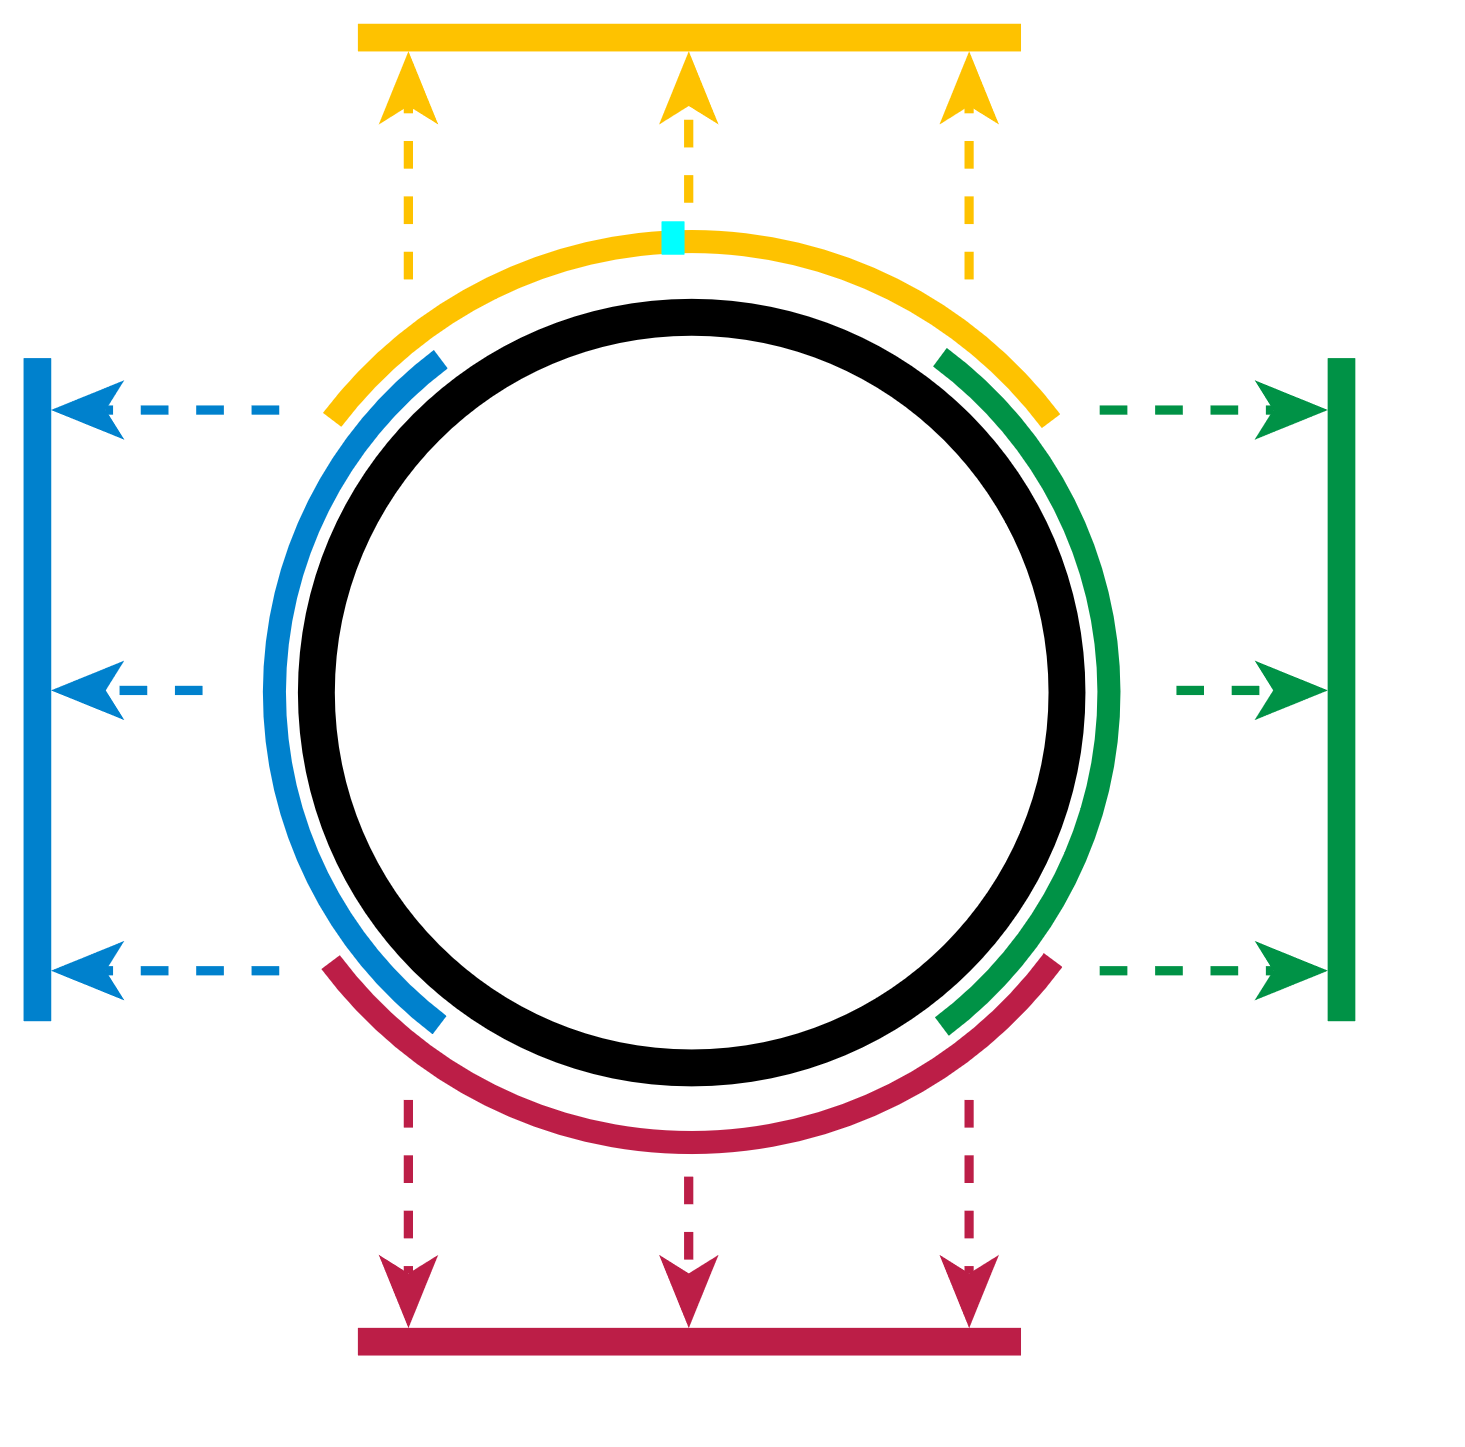
\includegraphics[width=0.5\textwidth]{img/circle.png}
  %   \caption{Подпись к картинке}
  %   \label{fig:img01}
  % \end{figure}

  % Chuck Norris sleeps with a pillow under his gun. Chuck Norris used to beat the shit out of his shadow because it was following to close. It now stands a safe 30 feet behind him. Look at fig.~\ref{fig:img01}. Chuck refers to himself in the fourth person. Chuck Norris once shattered the space-time continuum. He felt so bad, he put it back together. Chuck Norris has never blinked in his entire life. Never.

  

  % \begin{verbatim}
  %   #include <stdio.h>

  %   int main() {
  %     return 0;
  %   }
  % \end{verbatim}

  % Какой-то текст на русском языке.


  \printbibliography
  
\end{document}

